\section{Equitable Resource Allocation}

\subsection{Ausgangslage}

Verschiedene Typen von Anfragen werden von einem System behandelt. Hinzu kommt noch, dass diese unterschiedlich priorisiert sein können. Das System muss verhindern, dass es zusammenbricht, auch wenn nur ein Typ oder Priorität zur Überlastung neigt.

\subsection{Lösungsansatz}

Als Beispiel nehmen wir Anfragen an eine Firmen-Webseite. Einige wollen nur Informationen abgreifen, andere Bestellungen platzieren. Zudem sollen Anfragen von Angestellten mit höherer Priorität behandelt werden als jene von Kunden.
Würde man nun strikt nach Fresh Work before Stale (55) vorgehen, würde dies bedeuten, dass immer die neuste Anfrage verarbeitet wird. Dies kann aber dazu führen, dass höher priorisierte Anfragen tiefer priorisierten weichen müssen. Das führt dann zu einer Priority-Inversion, falls tiefer priorisierte Anfragen Ressourcen blockieren, welche von höher priorisierten benötigt werden.
Eine andere Lösung wäre, basierend auf den eingehenden und bereits vorhandenen Anfragen die Ressourcen zu verteilen. So können so viele Anfragen wie möglich mit den vorhandenen Ressourcen verarbeitet werden und Überlastungen blockieren nicht alle Typen und Prioritäten von Anfragen.

\subsection{Schlussfolgerung}

Bündle ähnliche Anfragen zusammen und stelle ihnen Ressourcen nach ihren Prioritäten bereit. Dies ermöglicht das Verarbeiten von allen Typen von Anfragen, auch wenn einige Gruppen zur Überlastung neigen.

\begin{figure}[H]
	\centering
	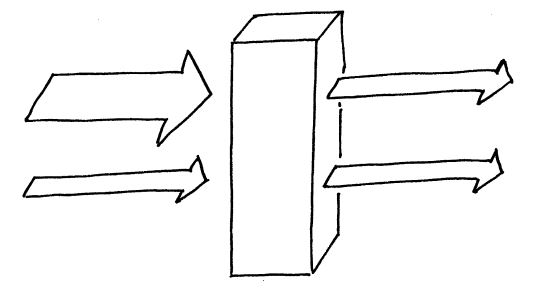
\includegraphics[width=\textwidth]{content/faulttolerance/images/EquitableResourceAllocation.JPG}
	\caption{EquitableResourceAllocation}
\end{figure}


\subsection{Verwandte Patterns}

Anwendung:
\begin{itemize}
	\item Queue for Resources (46)
\end{itemize}

